\documentclass[12pt,a4paper]{article}
\usepackage[margin=1in]{geometry}
\usepackage{graphicx}
\graphicspath{ {./images/} }
\usepackage{amsmath}
\usepackage{amssymb}
\usepackage{amsthm}
\usepackage{gensymb}
\usepackage{mathrsfs}
\usepackage{multicol}
\usepackage{tikz}
\usetikzlibrary{positioning}
\usepackage[autostyle]{csquotes}
\renewcommand{\baselinestretch}{0.8}
\setlength{\columnsep}{1cm}
\usepackage{xcolor} % font coloring
\usepackage{sectsty}
%\sectionfont{\color{red}}  % sets colour of sections
\setlength{\parindent}{-1em}
%\sectionfont{\color{red}}  % sets colour of sections
%\subsectionfont{\color{purple}}
%\subsubsectionfont{\color{blue}}

%% math macros
\newcommand{\R}{\mathbb{R}}
\newcommand{\Z}{\mathbb{Z}}
\newcommand{\N}{\mathbb{N}}
\newcommand{\C}{\mathbb{C}}
\newcommand{\Q}{\mathbb{Q}}
\newcommand{\W}{\mathbb{W}}
\newtheorem{thm}{Theorem}
\newtheorem{defn}{Definition}
\newtheorem{conv}{Convention}
\newtheorem{rem}{Remark}
\newtheorem{lem}{Lemma}
\newtheorem{cor}{Corollary}
\newtheorem{ex}{Example}
\newtheorem{pbm}{Problem}

%%% Coloring macros
\newcommand{\cred}[1]{\textcolor{red}{#1}}
\newcommand{\cblue}[1]{\textcolor{blue}{#1}}
\newcommand{\ccyan}[1]{\textcolor{cyan}{#1}}
\newcommand{\cgreen}[1]{\textcolor{green}{#1}}
\newcommand{\cyellow}[1]{\textcolor{yellow}{#1}}
\newcommand{\cpurple}[1]{\textcolor{purple}{#1}}
\newcommand{\corange}[1]{\textcolor{orange}{#1}}
%% custom colors
\definecolor{astral}{RGB}{46,116,181}
\definecolor{darkblue}{RGB}{50,76,168}
\definecolor{darkbrown}{RGB}{99,12,8}

\title{Group Theory \vspace{-2em}}
%\author{Hamjak Debbarma}
\date{\today}
\linespread{0.5}

\begin{document}
  \maketitle
  \section{Motivational Examples on Groups}
  Let $\Z$ be the set of all integers, performing binary operation $+$ on any two elements on $\Z$ we get the another integers, $3+2=5$ and $5+(-2)=3$. There exist a special element $0$ in $\Z$ such that adding any element with it, it produce the element itself. That is, let $n\in \Z$ then, $n+0=0+n=n$, $0$ is called the \textit{identity element} for addition. Every elements in $\Z$ has an inverse. i.e, if we add element and its inverse we get the identity element $5+(-5)=0$, $-3+3=0$. Since, addition is a binary operation how can we add three integers? We can first take two element add them then add with the other element i.e, $2+(3+4)=(2+3)+4=9$ this is called the associativity property.\\\\
  Formally, we can state the properties of addition on $\Z$ as -
  \begin{itemize}
    \item It is closed under addition.
    \item There is an identity element $0$ i.e, $\forall n\in \Z,\; n+0=0+n=n$
    \item Every elements has an inverse i.e, $\forall n\in \Z,\; n+(-n)=0$ 
    \item Addition is associative i.e, $\forall a,b,c\in \Z,\; a+(b+c)=(a+b)+c$
  \end{itemize}
  
  \begin{ex}
    Consider an equilateral $\triangle$ and consider a    `rotational symmetries' of $\triangle$ 
  \end{ex}
  \begin{center}
    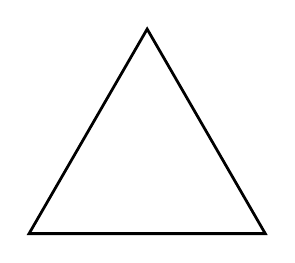
\begin{tikzpicture}
    \draw [line width=1pt] (0,0) -- (60:3) -- (3,0) -- cycle;
  \end{tikzpicture}
  \end{center}
  Let the rotational symmetries be $r1: 360^{\circ}\;r2: 120^{\circ}\;r3: 240^{\circ}$\\
  $\therefore G=\{r1,r2,r3\}$ consider a composition on $G$ That is, $r3\circ r2=r1$ ,  $r2\circ r2=r3$, $r2\circ r1=r2$ etc.\\ \\
  Then, the following properties hold -
  \begin{itemize}
    \item It is closed under composition
    \item There is an identity element $r1$. i.e, $\{360^{\circ},0^{\circ}\}$
    \item Every element has an inverse.
    \item Composition is Associative 
  \end{itemize}
  \begin{rem}
    Composition of a any function is associative. $(f\circ g)\circ h = f\circ (g\circ h)$
  \end{rem}
  
  %---------------------- 2 -----------------------------
  \section{Groups and its properties}
  \begin{defn}
    Let $(G,*)$ be an algebraic structures with binary operation $*$ then $G$ is called a group if it satisfy the following properties :
    \begin{itemize}
      \item Closure property i.e, $\forall a,b \in G\; a*b\in G$
      \item There exist an identity element $e$ s.t $a*e=e*a=a\; \forall a\in G$
      \item Every element $a\in G$ has an inverse $a^{-1}\in G$ s.t $a*a^{-1}=e$
      \item $*$ is Associative i.e, $\forall a,b,c \in G\; (a*b)*c=a*(b*c)$
    \end{itemize}
  \end{defn}
  \begin{defn}
    A group is $G$ is called Commutative or Abelian Group if it has commutative property i.e, $\forall a,b\in G\; a*b=b*a$
  \end{defn}
  \begin{ex}
    $(\Z,+)$, $(\R,+)$  $(\Q,+)$  $(\C,+)$ are all groups.
  \end{ex}
  \begin{ex}
    Is $(\Z,\times)$ group ? For any $a\in \Z$, $a^{-1}\notin \Z$ so, its not a group.
  \end{ex}
  \begin{ex}
    Is $(\Q,\times)$ group ? Clearly, $(\Q,\times)$ is not group but $\Q-\{0\}$ is a group.
  \end{ex}
  \begin{ex}
    $M_{n\times n}(\R)$ is a group under $+$.
  \end{ex}
  \begin{proof}
    $O$ or Null matrix is the identity for any $M_{n\times n}(\R)$, we have $-A$ for any matrix $A$ so inverse exist. Addition of matrices is associative by the property of matrices. 
  \end{proof}
  \begin{rem}
      $M_{n\times n}(\R)$ is not a group under multiplication.\\ But, $GLm = \{\text{set of all the invertible matrices over } \R\}$ is a group under multiplication.
  \end{rem}
  \begin{defn}
    A group $G$ is called finite group if the no. of elements in $G$ is finite.
  \end{defn}
  \begin{defn}
    If $G$ is finite group, then the \textbf{the order of $G$} is define to be the no. of elements of $G$. It is denoted as $o(G)$ or $|G|$
  \end{defn}
  \begin{defn}
    The \textbf{order of element} $a$ in $G$ is the smallest positive integer $n$ such that $a^n = e$. If  $a^n \neq e$ then $a$ has \textit{infinite order.}. Denoted as $o(a)=n$
  \end{defn}
  \begin{thm}[Cancellation Law]
    Let $G$ be a group and $a,b,c\in G$ such that $a*b=a*c \implies b=c$
  \end{thm}
   \begin{proof}
   Let $a^{-1}$ be the inverse of $a$ such that,
   \[
   \begin{aligned}
    a^{-1}(ab) &= a^{-1}(ac) \\
    (a^{-1}a)b &= (a^{-1}a)c    && \text{(by Associative law)}\\
    e*b &= e*c          && \text{($a^{-1}a=e$)} \\
    b &=c
   \end{aligned}
   \] 
   \end{proof}
  \begin{thm}
    A group $G$ has a unique identity element.
  \end{thm} 
  \begin{proof}
  Assume $G$ has two identities $e$ and $e^{\prime}$ then $e*e^{\prime}=e$ because $e^{\prime}$ is the identity element. But, $e*e=e$ then by above theorem we have $e*e=e*e^{\prime} \implies e =e^{\prime}$ 
  \end{proof}
  \begin{cor}
    Any elements of $G$ has unique inverse.
  \end{cor}
  \begin{proof}
    Let $a\in G$ suppose $a$ has two inverse $g$ and $h$ then, $a*g=a*h \implies g=h$
  \end{proof}
  \begin{lem}
    Let $G$ be Abelian and $a,b \in G$ such that $a*b=e$ then $b*a=e$
  \end{lem}
  \begin{proof} Let $a^{\prime}$ be the inverse of $a$. Then,
  \[
    \begin{aligned}
    a*b &= e \\
    a^{\prime}(ab) &= a^{\prime}*e \\
    e*b &= a^{\prime} \\
    b &= a^{\prime}
  \end{aligned}
  \]
  so, $b*a = a^{\prime}*a=e$
  \end{proof}
  \begin{thm} 
  If $a\in G$ then $(a^{-1})^{-1}=a$ and if $a,b\in G$ then $(ab)^{-1}=b^{-1}a^{-1}$
  \end{thm}
  \begin{proof}
    Let $e$ be the identity element.Then we $a*a^{-1}=e$ and $(a^{-1})^{-1}*a^{-1}=e$. Therefore, $(a^{-1})^{-1}*a^{-1}=a*a^{-1} \implies (a^{-1})^{-1}=a$ by cancellation law.\\
    Let $(ab)^{-1}*(ab)=e \forall \; a,b \in G$ and $b^{-1}a^{-1}*(ab)=a*a^{-1}*b*b^{-1}=e$. So, $(ab)^{-1}*(ab)=a*a^{-1}*b*b^{-1} = b^{-1}a^{-1}*(ab) \implies (ab)^{-1}= b^{-1}a^{-1}$ 
  \end{proof}
  \begin{lem}
    The identity is the only element whose order is $1$.
  \end{lem}
  \begin{proof}
    Consider, $o(a)=1$ for any $a\in G$ then $a^1=e \implies a=e$
  \end{proof}
  \begin{thm}
    Let $(G,*)$ be a group then the equation $a*x=b$ has a unique solution $x=a^{-1}*b$ and $y*a=b$ has unique solution $y=b*a^{-1}$
  \end{thm}
  \begin{proof}
    Let $x,x^{\prime} \in G$ be the two solution of eqn. $a*x=b$ then we have $a*x=b$ and $a*x^{\prime}=b$. Therefore,  $a*x=a*x^{\prime} \implies x=x^{\prime}$. So, $a*x=b$ has a unique solution $x$. Now, let $x=a^{\prime}*b$ then,
    $$a*x=(a*a^{\prime})b=e*b=b$$
    The second part can be proved using same arguments.
  \end{proof}
  \begin{pbm}
    Let $G=\{\frac{a}{b} \in \Q | gcd(a,b)=1 \;\text{and}\; 5\mid b \}$. Is $G$ a group under $+$?
  \end{pbm}
  \begin{proof}[Soln.]
    Clearly, closure property does not hold on $G$\\
    e.g, $\frac{2}{5} + \frac{3}{5} = \frac{5}{5} = 1 \notin G$
  \end{proof}
  \begin{pbm}
    Let $G=\{\frac{a}{b} \in \Q | gcd(a,b)=1 \;\text{and}\; 5 \nmid b \}$. Is $G$ a group under $+$?
    \begin{proof}[Soln.]
      Let $\frac{a}{b},\frac{c}{d} \in G$  then by the divisiblity property if $5\nmid b$ and $5\nmid d$ then $5\nmid bd$ .So,
      $\frac{a}{b} + \frac{c}{d} = \frac{ad+bc}{bd} \in G$. Clearly, $0$ is the identity and $\frac{-p}{q}$ is the inverse for any $\frac{p}{q}\in G$. Therefore, $(G,+)$ is a group. Furthermore, it is also Commutative group as $\frac{a}{b} + \frac{c}{d} = \frac{ad+bc}{bd} = \frac{c}{d}+\frac{a}{b}$
    \end{proof}
  \end{pbm}
  %------------ 3 ----------------------------
  \section{Groupoid, Semi-Group and Monoid}
  \begin{defn}
    Let $(S,*)$ be an algebraic structures in which $S$ is non-empty set and $*$ is binary operation define on $S$. Such structure $(S,*)$ is called \textbf{Groupoid}.
  \end{defn}
  \begin{defn}
   An algebraic structure  $(S,*)$ is called a \textbf{semi-group} if the operation $*$ is closed and Associative.
  \end{defn}
  \begin{defn}
    A semi-group containing an identity element is called \textbf{monoid.}
  \end{defn}
  \begin{pbm}
    Let $(A,*)$ be a semigroup. Show that for $a,b,c \in A$ if $a*c=c*a$ and $b*c=c*b$ then $(a*b)*c=c*(a*b)$
  \end{pbm}
  \begin{proof}[Soln.]
  Since, $A$ is semigroup it is Associative. We have $$(a*b)*c=a*(b*c)=a*(c*b)=(a*c)*b \implies c*(a*b)$$
  \end{proof}
  \begin{pbm}
    Let $(\{x,y\},\circ)$ be a semigroup where $xx=y$ show that $xy=yx$ and $yy=y$
  \end{pbm}
  \begin{proof}[Soln.]
  \[
    \begin{aligned}
    xy &= x(xx)   && \text{$[xx=y]$} \\
    &= (xx)y \\
    &= yx
    \end{aligned}
  \]
  Since, $(\{x,y\},\circ)$ is closed we have two cases -\\
  \textbf{case $1$: } $xy=x$
  \[
  \begin{aligned}
    yy &= (xx)y \\
    &= x(xy)    && \text{$[xy=x]$} \\
    &= xx     && \text{$[xx=y]$} \\
    &= y
  \end{aligned}
  \]
  \textbf{case $2$: } $xy=y$
  \[
  \begin{aligned}
    yy &= (xx)y \\
    &= x(xy)    && \text{$[xy=y]$} \\
    &= xy  \\
    &= y
  \end{aligned}
  \]
  \end{proof}
  % ----------- 4 ----------------------------
  \section{Subgroups}
  \begin{defn}
    Let $(G,*)$ be a group. A subgroup $H$ of $G$ is a subset of $G$ which has the following properties.
    \begin{itemize}
      \item $H$ is closed under $*$
      \item $e\in H$
      \item if $a\in H \implies a^{-1}\in H$
    \end{itemize}
    Denoted as $H \leq G$
  \end{defn}
  \begin{rem}
    If $H \leq G$ then $H$ is also a group under same operation of $G$.
  \end{rem}
  \begin{lem}
    Every subgroup of $\Z$ is of the form $n\Z$ for any $n \in \Z^{+}$
  \end{lem}
  \begin{proof}
    Let $H$ be any arbitrary subgroup of $\Z$. Then, there exist $m\in H$ such that $m^{\prime}\in H$ since, $H$ is a group itself. If $H=\{0\}$ then $H=0\Z$. Suppose, $H \neq\{0\}$ so, $H$ contains an integer $n>0$ (why?) if $n>0$ then we are done. But if $n<0$ then $n^{\prime}>0 \implies n\in H \implies n^{\prime}\in H $. This shows that positive integer exist in $H$. Let $n$ be the least positive integer of $H$. Then, we claim $H=n\Z$. Clearly, $n\Z \subseteq H$. Now, let $k\in H$ such that $k \leq n$ then, dividing $k$ by $n$ we get $k=nq+r$, for some $r,q\in \Z$ where, $0\leq r < n$, $k-nq=r \implies k-nq=0$ since $r<n$ and $n$ is the least element. So, $k=nq, k\in n\Z$. That means, $H \subseteq n\Z \implies H=n\Z$
  \end{proof}
  \begin{lem}
    The necessary and sufficient condition for $H$ to be the subgroup of $G$ is whenever $x,y\in H$ then $x*y^{-1} \in H$.
  \end{lem}
  \begin{proof}
    Since, $H \neq \varnothing, \exists x\in H \implies x*x^{-1}\in H \implies e\in H$. So, identity and inverse exist in $H$ for each $x\in H$. Let $x,y \in H$ we have $y^{-1}\in H$ so $x*(y^{-1})^{-1}=x*y\in H$ hence, Closure property hold. Therefore, $H \leq G$.
  \end{proof}
  \begin{lem}
    Let $H_{1},H_{2} \leq G$ then $H_{1} \cap H_{2} \leq G$
  \end{lem}
  \begin{proof}
    Clearly,$H_{1} \cap H_{2}=\varnothing$ because $e\in H_{1},H_{2}$
    let $a\in H_{1} \cap H_{2} \implies a\in H_{1} \text{and}\;H_{2}$,
    $b\in H_{1} \cap H_{2} \implies b\in H_{1} \text{and}\;H_{2}$. Since, $b\in H_{1}\implies b^{-1}\in H_{1}$ so, $a*b^{-1}\in H_{1}$ similarly, $b\in H_{2}\implies b^{-1}\in H_{2}$ so, $a*b^{-1}\in H_{2}$. Therefore, $a*b^{-1}\in H_{1}\cap H_{2}$.
  \end{proof}
  %------------ 5 ---------------------------
  \section{Cyclic Groups}
  \begin{defn}
    Let $G$ be a group, $a\in G$ if all the elements of $G$ are in the form $a^n\in G$ for some $n\in \Z$. Then, $G$ is called the cyclic group. $a$ is the generator of the group. \\
    Denoted as $G=<a> = \{\dots a^{-2},a^{-1},e,a^{1},a^{2},\dots\}$
  \end{defn}
  \begin{lem}
    If $x$ is the generator of $G$ then $x^{-1}$ is also a generator.
  \end{lem}
  \begin{proof}
    Since, $G=<x>$ then $G$ is of the form $x^n$ for some $n\in \Z$ then $x^n=x^{(-1)-n}, x^{-1}\in G,n^{-1}\in \Z$ 
  \end{proof}
  \begin{lem}
    Every cyclic group is Abelian
  \end{lem}
  \begin{proof}
    Let $a^r,a^s\in G$ for some $r,s\in \Z$ we have 
    $$
    \begin{aligned}
      a^r*a^s &=\underbrace{(a*a*a*\dots *a)}_{r}*\underbrace{(a*a*a*\dots *a)}_{s}\\
          &= \underbrace{(a*a*a*\dots *a)}_{r+s} \\
          &=a^{r+s} \implies a^s*a^r
    \end{aligned}     
    $$
  \end{proof}
   \begin{rem}
    Every Abelian is not necessarily a cyclic.
   \end{rem}
  \begin{lem}
    If a cyclic group $G$ is generated by an element of order $n$ then $a^m$ is a generator of $G$ iff $gcd(n,m)=1$.
  \end{lem}
  \begin{thm}[Definition of Cyclic Group]
    Let $G$ be a group and $a$ be any element in $G$ then, the set $<a>=\{a^k:k\in \Z\}$ is a subgroup of $G$. Furthermore, $<a>$ is the smallest subgroup of $G$ that contain $a$.
  \end{thm}
  \begin{proof}
    The identity is in $<a>$ since, $a^0=e$.If $g$ and $h$ are any two elements in $<a>$, then by definition of $<a>$ we can write $g=a^m$ and $h=a^n$ for some $n,m\in \Z$. So, $gh=a^ma^n=a^{m+n} \in <a>$. Finally, if $g=a^m \in <a> \implies g^{-1}=a^{-n}\in <a>$ hence, inverse also exist in $<a>$. That implies, $<a> < G$.Therefore, $<a>$ is the smallest subgroup of $G$ that contain $a$. 
  \end{proof}
  \begin{lem}
    Every subgroup of a cyclic group is also cyclic.
  \end{lem}
  %-----------6------------------------------
  \section{Homomorphism and Isomorphism}
  %------------7-----------------------------
  \section{Cosets and Langrange's Theorem}
  %-------------8----------------------------
  \section{Permutation Groups}
  %------------9----------------------------
  \section{Group Actions}
\end{document}